\section{Implementation}
\label{sec:implementation} 

We describe a implementation of the side-channel attack on CPU usage statistics. 
We implemented prototype application which monitors CPU usage statistics of other application running on an Android device.
Our prototype application calls \term{top} system call periodically and generates an accumulated log of Netflix application running the device. 
However, a target of monitoring is not confined to Netflix.
Our prototype can monitor any applications running on the Android device. 
Figure \ref{fig:prototype_screenshot} shows a screenshot of our prototype implementation. 
Each line of log consists of \term{pid}, \term{CPU usage}, \term{State}, \term{Number of threads}, \term{Virtual set size}, \term{Resident set size}, \term{Foreground/Background}, \term{User ID} and \term{Process name}. 

\begin{figure}[!h]
\centering
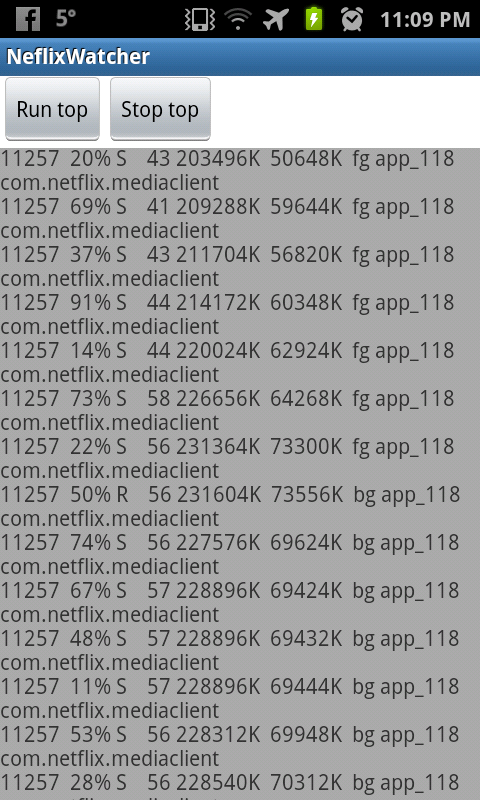
\includegraphics[scale=0.35]{Figures/netflix_watcher_screenshot2}
\caption{Screenshot of prototype implementation}
\label{fig:prototype_screenshot}
\end{figure}

The most important feature of our prototype implementation is that collecting CPU usage statistics of other applications does not require any permission from a user. 
Android permissions required by applications are categorized into 2 categories: \term{Normal} and \term{Dangerous}.
(Actually there exist two more permission categories granted only to system application but these are not our concern.)
Generally, \term{Normal} permission is not directly related to user privacy but \term{Dangerous} permission is. 
Upon installing an application which requires \term{Normal} or \term{dangerous} permissions, a user is notified so that he may refuse to install the application. 
Since our prototype does not require any kind of permission from users, it can be perceived to be a non-malicious application by users. 
Moreover, the prototype can be embedded into other Android applications transparently to users. 
The side-channel attack exploiting CPU usage of an application, therefore, can be performed covertly.

Although our prototype does not require any permission, a commodity-level implementation would need an access to the Internet in order to transmit collected CPU usage statistics. 
Since Internet access permission is categorized as \term{Dangerous}, it would harm the transparency of our prototype. 
However, \cite{Chia:2012} reveals that about 77\% of 650 popular Android applications requires an access to the Internet. 
Therefore, it should be still reasonable that our implementation can be easily embedded into other Android application transparently to users. 


